\documentclass{beamer}
\usetheme{Madrid}

\usepackage{amssymb}
\usepackage{apacite}
\usepackage{natbib}
\usepackage{bibentry}
\usepackage{graphicx}
\usepackage{booktabs}

\usepackage{hyperref}
\usepackage{subcaption}
\usepackage{amsmath}
\usepackage{lipsum}

\title{Deep Reinforcement Learning Tutorials}
\author{Wilbert Santos Pumacay Huallpa}

\begin{document}

\begin{frame}
    \titlepage
\end{frame}

\begin{frame}
    \frametitle{Logistics}
    Outline of the sessions:
    \begin{itemize}
        \item Tutorial 0: Introduction
        \item Tutorial 1: Tabular value-based methods
        \item Tutorial 2: Value-based methods with Function Approximation
        \item Tutorial 3: Policy Optimization and Policy Gradient methods
    \end{itemize}

    \pause

    Some code (hopefully):
    \begin{itemize}
        \item Tutorial 0: OpenAI-Gym.
        \item Tutorial 1: MC-control, SARSA and Q-learning (Tabular).
        \item Tutorial 2: Deep Q-learning (DQN)
        \item Tutorial 3: Behaviour cloning, Vanilla Policy Gradients, DDPG.
    \end{itemize}
\end{frame}

\begin{frame}
    \frametitle{Outline for today}
    \begin{itemize}
        \item Introduction to Reinforcement Learning
            \begin{itemize}
                \item What is Reinforcement Learning?
                \item Defining the problem.
                \item Defining the solution.
            \end{itemize}
        \item Introduction to OpenAI-Gym.
    \end{itemize}
\end{frame}

%%%%%%%%%%%%%%% Section 1 - Intro to RL %%%%%%%%%%%%%%%%%%%
\section{Introduction to Reinforcement Learning}

%% {
%%     \setbeamercolor{background canvas}{bg=black}
%%     \begin{frame}[plain,c]
%%         \begin{center}
%%         \Huge {\color{white} A quick introduction to Reinforcement Learning}
%%         \end{center}
%%     \end{frame}
%% }

%% * Introduce in a high level what RL is about
%% * Give some examples about its successes 
%% * Give some preliminary hints about the differences to Supervised learning
%% * Give some preliminary hints about what usually can go wrong

\subsection{What is Reinforcement Learning?} \title{What exactly is Reinforcement Learning?} \author{} \date{}
\begin{frame}[plain,c]
    \titlepage
\end{frame}

\begin{frame}
    \frametitle{Reinforcement Learning (RL)}
    \begin{itemize}
        \item A learning approach in which \textbf{agents learn by}
              \textbf{trial and error}.
            \begin{figure}
                \centering
                
\includegraphics[width=0.25\textwidth]{./imgs/img_rl_environment_agent.png}
            \end{figure}
        \pause
        \item A framework for \textbf{sequential} decision making and learning under
              \textbf{uncertainty}.
            \begin{figure}
                \centering
                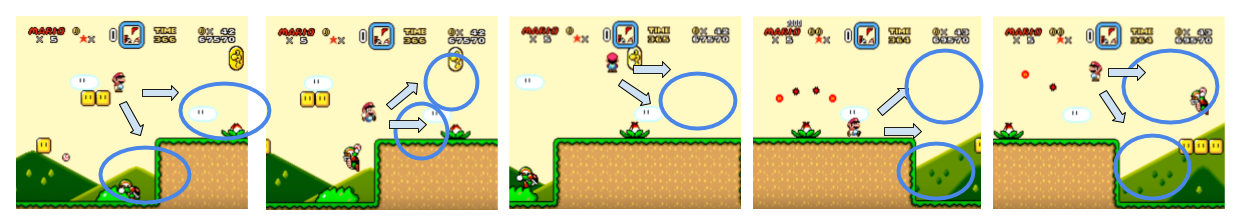
\includegraphics[width=0.9\textwidth]{./imgs/img_sequential_mario.png}
            \end{figure}
    \end{itemize}
\end{frame}

\begin{frame}
    \frametitle{Some RL success stories}
    \begin{figure}[!ht]
        \centering
        \begin{subfigure}{0.4\textwidth}
            \centering
            \href{https://youtu.be/TmPfTpjtdgg}{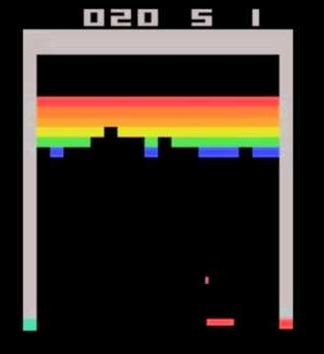
\includegraphics[width=0.6\textwidth]{./imgs/img_motivation_dqn_atari.png}}
            \caption{\cite{DQNAtari}}
        \end{subfigure}
        \begin{subfigure}{0.4\textwidth}
            \centering
            \href{https://youtu.be/jGyCsVhtW0M}{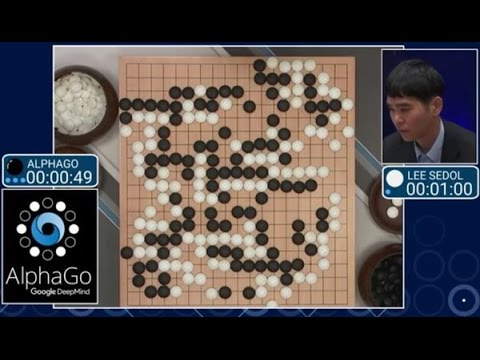
\includegraphics[width=0.7\textwidth]{./imgs/img_motivation_alpha_go.png}}
            \caption{\cite{AlphaGo}}
        \end{subfigure}

        \centering
        \begin{subfigure}{0.4\textwidth}
            \centering
            \href{https://youtu.be/hx_bgoTF7bs}{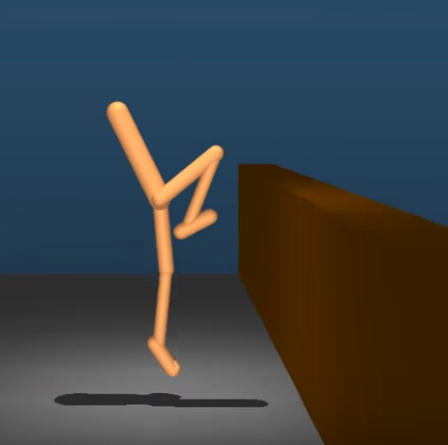
\includegraphics[width=0.6\textwidth]{./imgs/img_motivation_locomotion.png}}
            \caption{\cite{DeepmindEmergenceLocomotion}}
        \end{subfigure}
        \begin{subfigure}{0.4\textwidth}
            \centering
            \href{https://youtu.be/vppFvq2quQ0}{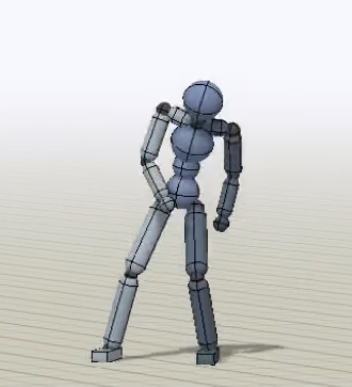
\includegraphics[width=0.6\textwidth]{./imgs/img_motivation_deepmimic.png}}
            \caption{\cite{DeepMimic}}
        \end{subfigure}
    \end{figure}
\end{frame}

%% * Introduce the RL setup
%% * Define formally the RL setup using MDPs
%% * Give some examples of MDPs
%% * Give some hints about POMDPs

\subsection{The problem} \title{Defining the RL framework} \author{} \date{}
\begin{frame}[plain,c]
    \titlepage
\end{frame}

\begin{frame}
    \frametitle{Agent-environment interaction}
    \begin{figure}
        \centering
        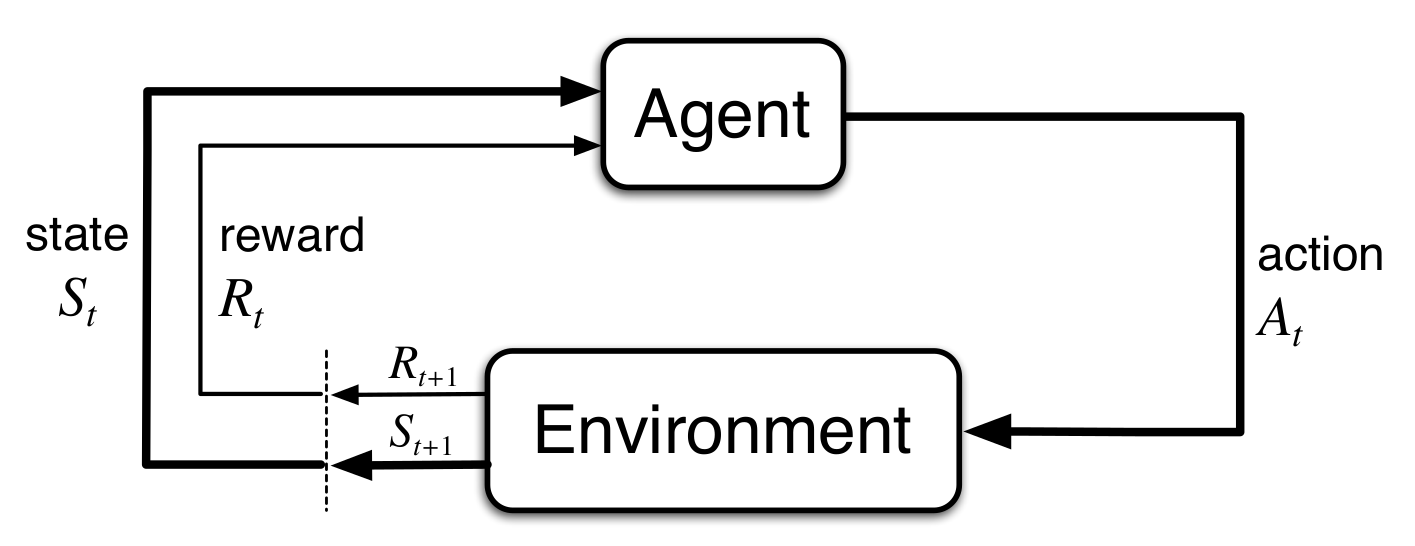
\includegraphics[width=0.6\textwidth]{./imgs/img_rl_loop.png}
        \caption{RL interaction loop \cite{RLbook}}
    \end{figure}

    \pause

    \begin{itemize}
        \item State $s_{t}$: configuration of the world. \pause
        \item Action $a_{t}$: available ways to act in the world. \pause
        \item Environment: dynamics of the world the agent lives in. \pause
        \item Reward $r_{t+1}$: reward given by the world for our transition. \pause
        \item Next state $s_{t+1}$: next state the agent lands in the world.
    \end{itemize}
\end{frame}

\begin{frame}
    \frametitle{Example: Locomotion}
    \begin{figure}
        \centering
        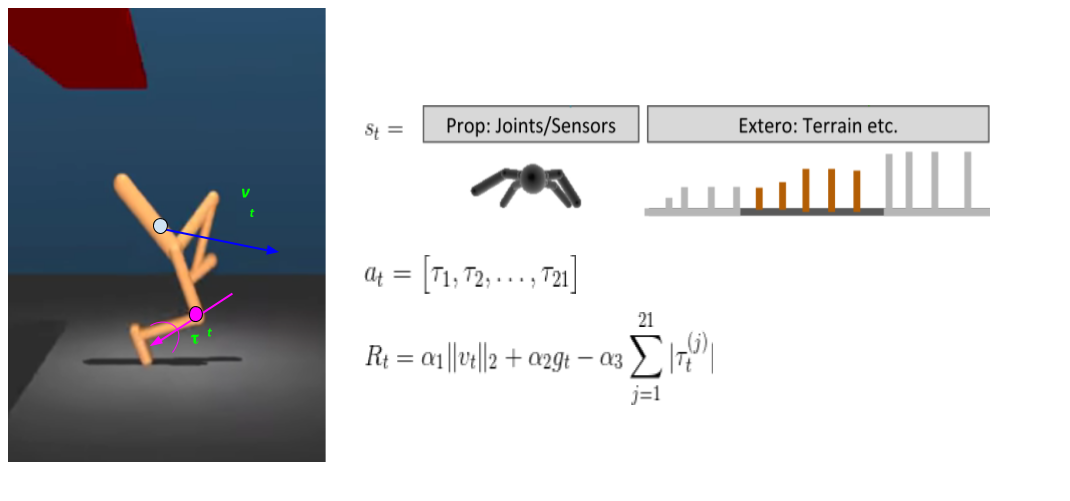
\includegraphics[width=\textwidth]{./imgs/img_rl_mdp_locomotion.png}
    \end{figure}
\end{frame}

\begin{frame}
    \frametitle{Example: Atari games}
    \begin{figure}
        \centering
        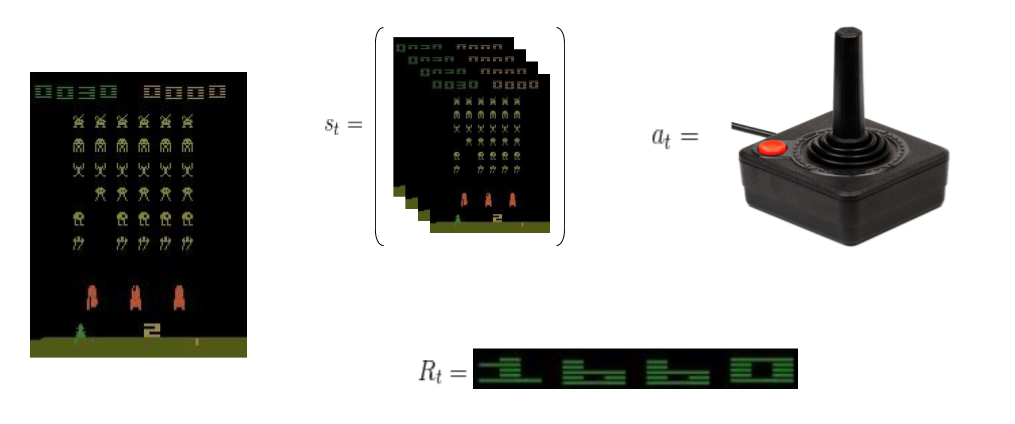
\includegraphics[width=\textwidth]{./imgs/img_rl_mdp_atari.png}
    \end{figure}
\end{frame}

\begin{frame}
    \frametitle{Mathematical Formulation: Markov Decision Processes}
    \begin{block}{Markov Decision Process}
        A Markov Decision Process is a mathematical framework for sequential
        decision making under uncertainty, defined by the tuple $(S,A,P,R)$ :
        \begin{itemize}
            \item $S=\left \{ s \right \}$: State space.
            \item $A=\left \{ a \right \}$: Action space.
            \item $P=p(s'|s,a)$: Transition model.
            \item $R(s)$ or $R(s,a)$ or $R(s,a,s')$: Reward function.
        \end{itemize}
    \end{block}

    \pause

    \begin{figure}
        \centering
        \begin{subfigure}{0.18\textwidth}
            \centering
            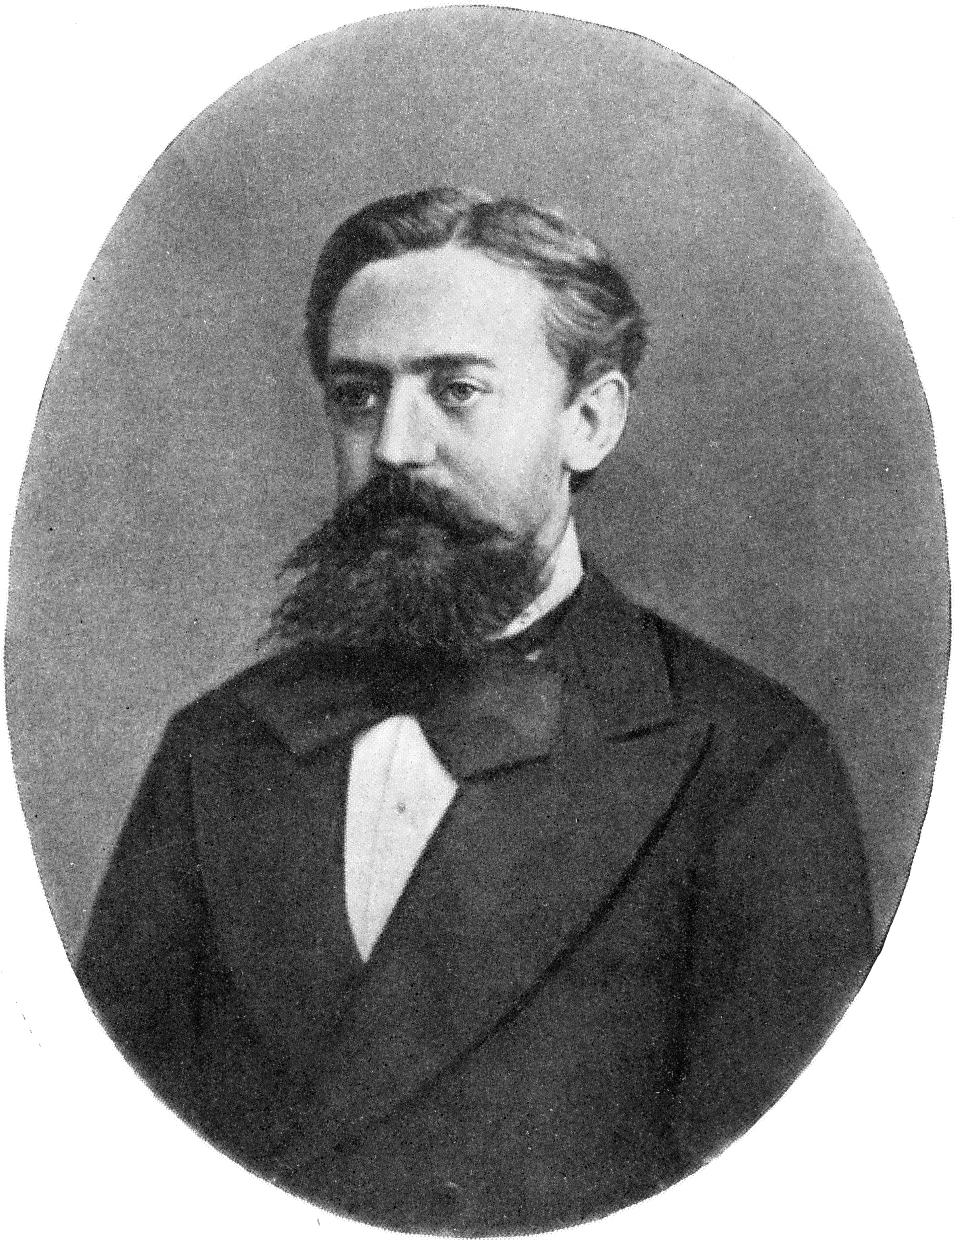
\includegraphics[width=0.9\textwidth]{./imgs/img_rl_mdp_andrey_markov.png}
            \caption{Andrey Markov}
        \end{subfigure}
        \hspace{0.1\textwidth}
        \begin{subfigure}{0.4\textwidth}
            \centering
            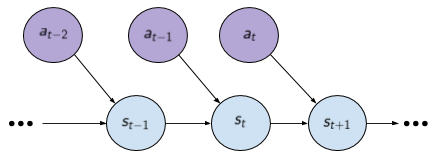
\includegraphics[width=0.9\textwidth]{./imgs/img_rl_mdp_graphical_model.png}
            \caption{Graphical model of an MDP}
        \end{subfigure}
    \end{figure}
\end{frame}

\begin{frame}
    \frametitle{A simple recycling robot MDP}
    \begin{figure}
        \centering
        \begin{subfigure}{0.45\textwidth}
            \centering
            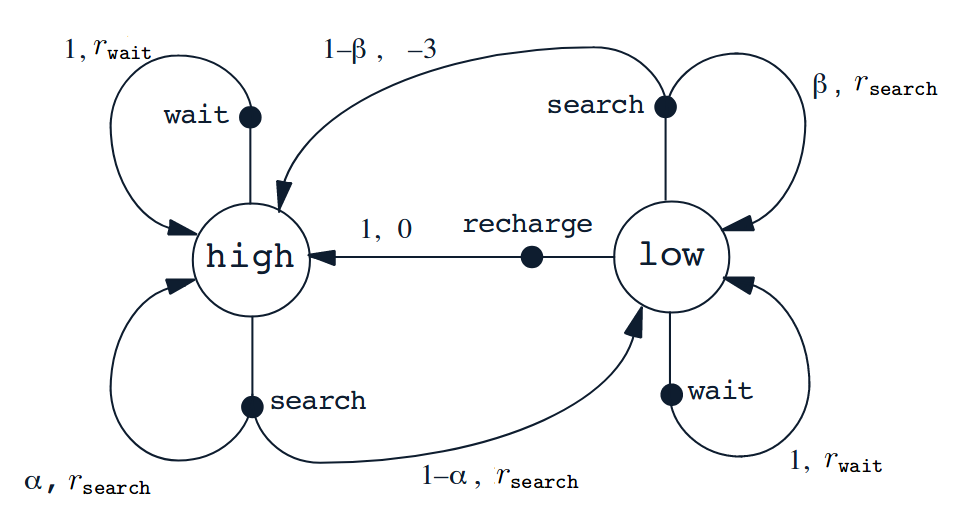
\includegraphics[width=0.9\textwidth]{./imgs/img_rl_mdp_robot_cleaner_1.png}
            \caption{MDP of a recycling robot}
        \end{subfigure}
        \pause
        \begin{subfigure}{0.45\textwidth}
            \centering
            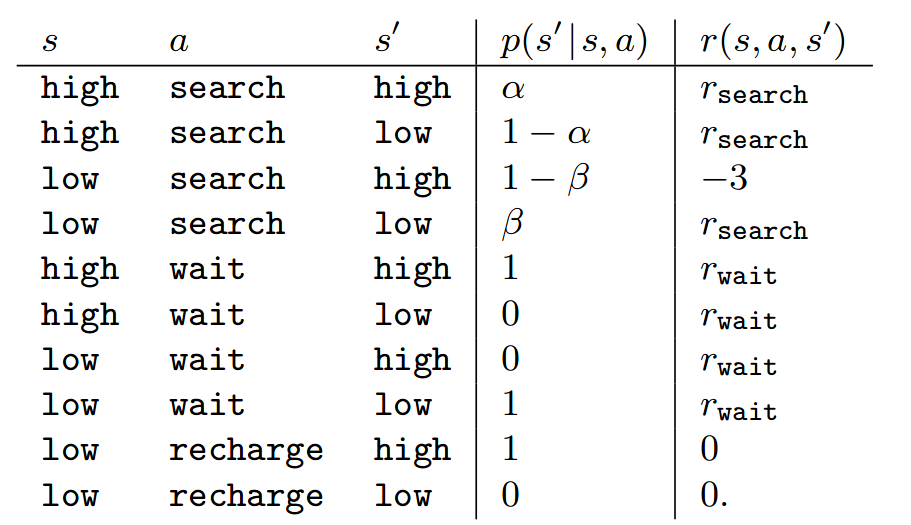
\includegraphics[width=0.9\textwidth]{./imgs/img_rl_mdp_robot_cleaner_2.png}
            \caption{Transition dynamics of the recycling robot MDP}
        \end{subfigure}
    \end{figure}
\end{frame}

\begin{frame}
    \frametitle{Another simple example}
    \begin{figure}
        \centering
        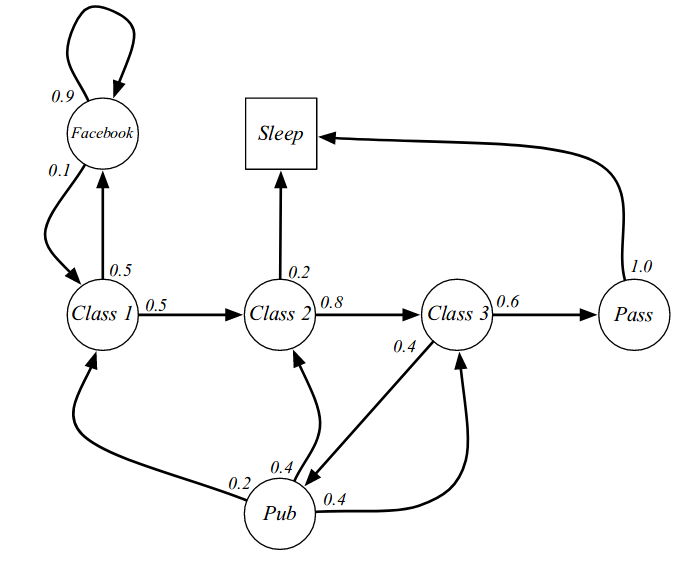
\includegraphics[width=0.5\textwidth]{./imgs/img_rl_mdp_student_example.png}
        \caption{Another example of an MDP}
    \end{figure}
\end{frame}

\begin{frame}
    \frametitle{Does the Markov assumption hold?}
    \begin{itemize}
        \item In general, we don't always have access to the full state
              of the environment $s_{t}$.
        \item Instead, we usually just have access to some observation
              $o_{t}$ (generated from $s_{t}$) which gives less information.
        \item Because of this, we might not be able to recover the full state
              of the environment from the observations we have.
    \end{itemize}

    \pause

    \begin{figure}
        \centering
        \begin{subfigure}{0.3\textwidth}
            \centering
            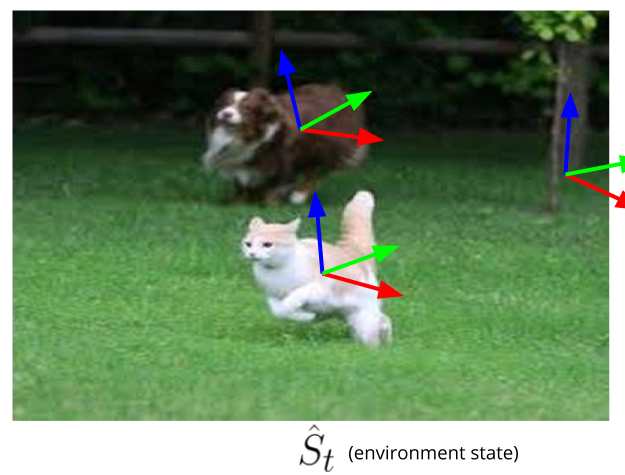
\includegraphics[width=0.9\textwidth]{./imgs/img_rl_pomdp_example_2.png}
        \end{subfigure}
        \begin{subfigure}{0.3\textwidth}
            \centering
            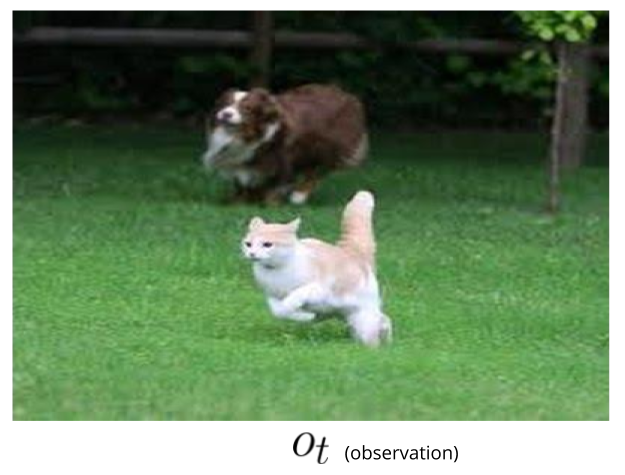
\includegraphics[width=0.9\textwidth]{./imgs/img_rl_pomdp_example_1.png}
        \end{subfigure}
        \begin{subfigure}{0.3\textwidth}
            \centering
            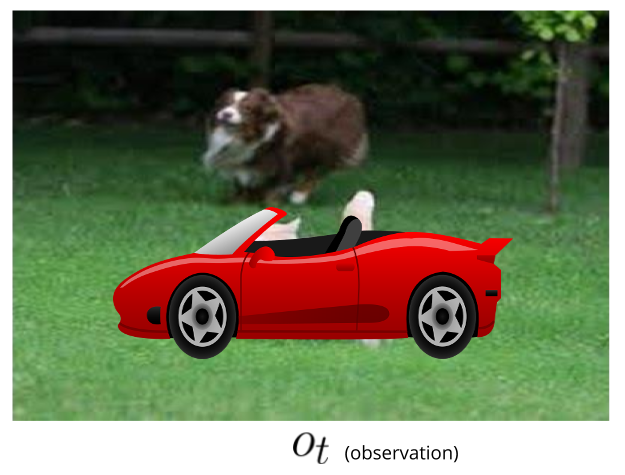
\includegraphics[width=0.9\textwidth]{./imgs/img_rl_pomdp_example_3.png}
        \end{subfigure}
    \end{figure}
\end{frame}

\begin{frame}
    \frametitle{Partially Observable MDPs (POMDPs)}
    \begin{block}{Partially Observable Markov Decision Processes (POMDP)}
        A POMDP is an MDP with hidden states defined by the following:
        \begin{itemize}
            \item $S=\left \{ s \right \}$: State space.
            \item $A=\left \{ a \right \}$: Action space.
            \item $\Omega=\left \{ o \right \}$: Observation space.
            \item $P=p(s'|s,a)$: Transition model.
            \item $R(s)$ or $R(s,a)$ or $R(s,a,s')$: Reward function.
            \item $Z=p(o|s)$: Observation model
        \end{itemize}
    \end{block}

    \pause

    \begin{figure}
        \centering
        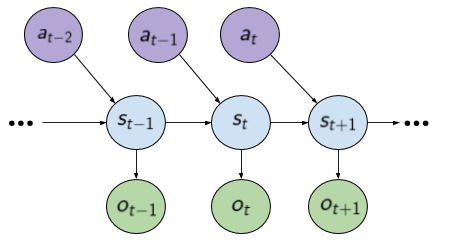
\includegraphics[width=0.4\textwidth]{./imgs/img_rl_pomdp_graphical_model.png}
    \end{figure}
\end{frame}

\begin{frame}
    \frametitle{What's the objective of the agent?}
    \begin{block}{Try 1: Maximize reward?}
        \begin{itemize}
            \item $\max r_{t+1}$ ???
            \pause
            \item Not really, as doing only good things \textbf{now} does
                  not guarantee that we do well in the long-run.
        \end{itemize}
    \end{block}
    \pause
    \begin{block}{Try 2: Maximize sum of rewards?}
        \begin{itemize}
            \item $\max \sum_{t=1}^{T} r_{t}$
            \pause
            \item Almost. Recall that the environment might be stochastic.
        \end{itemize}
    \end{block}
    \pause
    \begin{block}{RL objective}
        \begin{equation*}
            \max \mathbb{E} \left \{ \sum_{t=1}^{T} r_{t} \right \}
        \end{equation*}
    \end{block}
\end{frame}

%% * Define trajectories
%% * Define returns
%% * Define policies
%% * Define State-value functions
%% * Define Action-value functions
%% * Present the types of solution methods

\subsection{The solution} \title{Defining the solutions} \author{} \date{}
\begin{frame}[plain,c]
    \titlepage
\end{frame}

\begin{frame}
    \frametitle{Policies $\pi$}
    \begin{itemize}
        \item Policies are mappings that from states $s_{t}$ that the agent
              might currently be in, to actions $a_{t}$ that the agent should
              take in those states.
              \begin{figure}
                \centering
                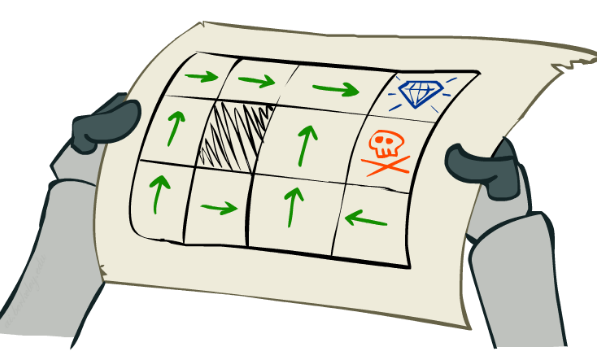
\includegraphics[width=0.5\textwidth]{./imgs/img_rl_policies.png}
              \end{figure}
        \pause
        \item These mappings could either be \textbf{Deterministic} (map a state
              to a single action) or \textbf{Stochastic} (map a state to a distribution
              over actions).
    \end{itemize}
\end{frame}

\begin{frame}
    \frametitle{Deterministic vs Stochastic Policies}
    \begin{figure}
        \centering
        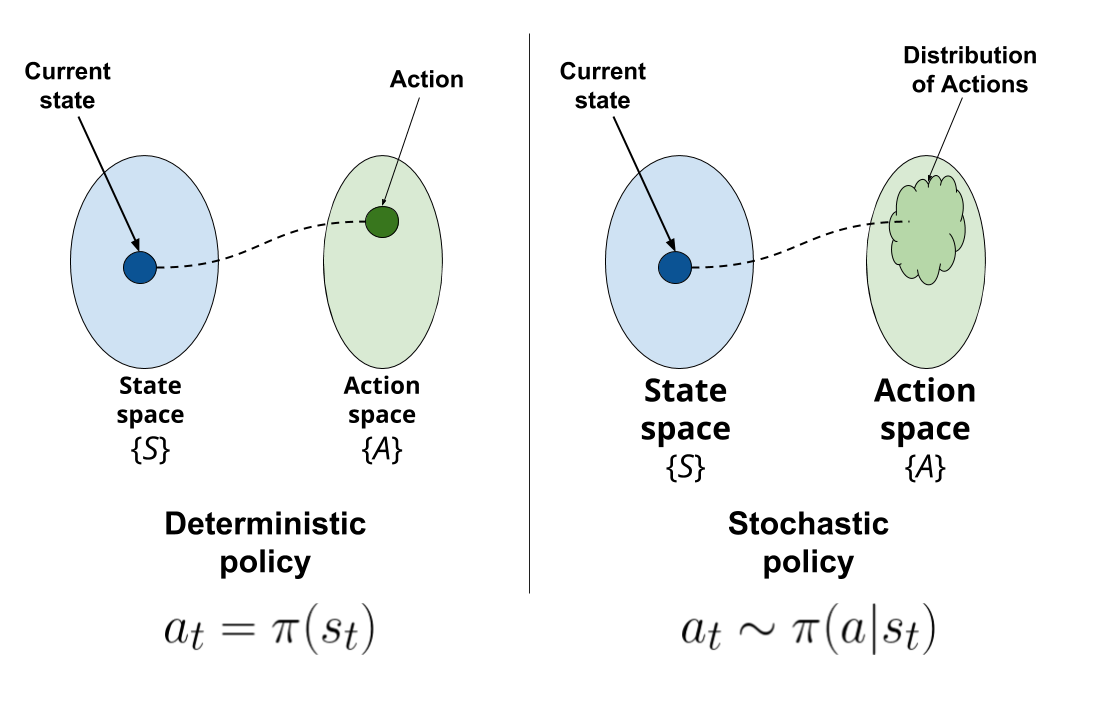
\includegraphics[width=0.9\textwidth]{./imgs/img_rl_policies_types.png}
    \end{figure}
\end{frame}

\begin{frame}
    \frametitle{Some more definitions}
    \begin{block}{Trajectories}
        A \textbf{trajectory} $\tau$ is a sequence of states-actions-rewards generated by running
        a policy in the environment.
        \begin{equation*}
            \tau = (s_{0},a_{0},r_{1},s_{1},a_{1},r_{2},\hdots)
        \end{equation*}
    \end{block}
    \pause
    \begin{block}{Returns}
        A \textbf{return} $G_{t}$ is the cummulative reward obtained from a given timestep
        onwards.
        \begin{equation*}
            G_{t} = \sum_{t'=1}^{T} r_{t' + t}
        \end{equation*}
    \end{block}
\end{frame}

\begin{frame}
    \frametitle{Optimal policies}
    \begin{block}{RL-objective}
        We can define the RL-objective using the previous concepts as follows:
        \begin{equation*}
            \pi^{*} = \arg \max_{\pi} \mathbb{E}_{\pi} \left \{ G_{t} \right \}
        \end{equation*}
        Where the policy $\pi^{*}$ is called the optimal policy.
    \end{block}
    \pause
    \begin{block}{Optimal Policy}
        An Optimal Policy $\pi^{*}$ is a policy (there could be many) that for any
        state $s \in S$, it gets more expected return than any other policy $\pi$
        at that same state $s$.
        \begin{equation*}
            \mathbb{E}_{\pi^{*}} \left \{ G_{t} | s_{t} = s \right \} \geq
            \mathbb{E}_{\pi} \left \{ G_{t} | s_{t} = s \right \}; \forall \pi, \forall s \in S
        \end{equation*}
    \end{block}
\end{frame}

\begin{frame}
    \frametitle{State-value functions}
    \begin{itemize}
        \item As explained earlier, the objective of the agent is to find the policy
              that for any state $s \in S$ it picks the action that maximizes expected
              return $\mathbb{E}_{\pi}\left \{ G_{t} | s_{t} = s \right \}$

        \pause

        \item Let's define the expected return starting at state $s_{t}=s$ and
              following policy $\pi$ as the \textbf{State-Value Function} $V_{\pi}(s)$.
              \begin{equation*}
                V_{\pi}(s) = \mathbb{E}_{\pi} \left \{ G_{t} | s_{t} = s \right \}
              \end{equation*}
    \end{itemize}
\end{frame}

\begin{frame}
    \frametitle{State-value functions}
    \begin{figure}
        \centering
        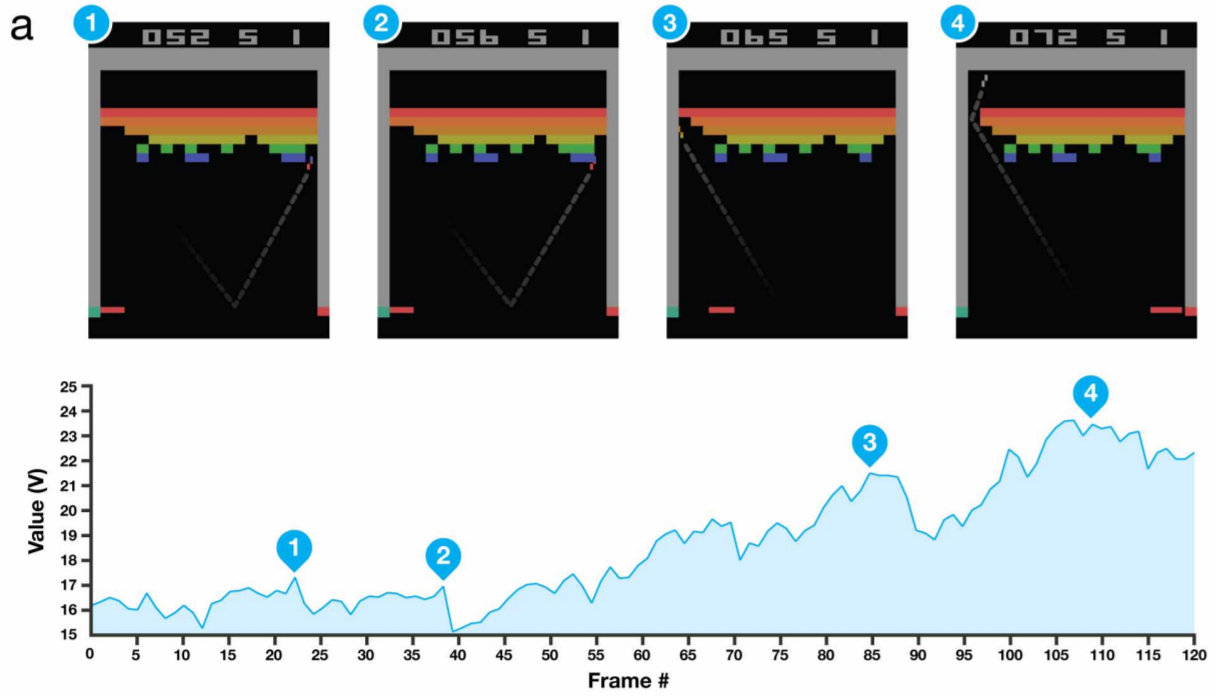
\includegraphics[width=0.9\textwidth]{./imgs/img_rl_vfunction_intuition.png}
    \end{figure}
\end{frame}

\begin{frame}
    \frametitle{Action-value functions}
    \begin{itemize}
        \item Similarly, we can define a function that tells us how well an action 
              $a_{t}=a$ would be if we take it in state $s_{t}=s$ and then follow
              the policy $\pi$ onwards.

        \pause

        \item We define this function as the \textbf{Action-Value Function} $Q_{\pi}(s,a)$
              \begin{equation*}
                Q_{\pi}(s,a) = \mathbb{E}_{\pi} \left \{ G_{t} | s_{t} = s, a_{t} = a \right \}
              \end{equation*}
    \end{itemize}
\end{frame}

\begin{frame}
    \frametitle{Action-value functions}
    \begin{figure}
        \centering
        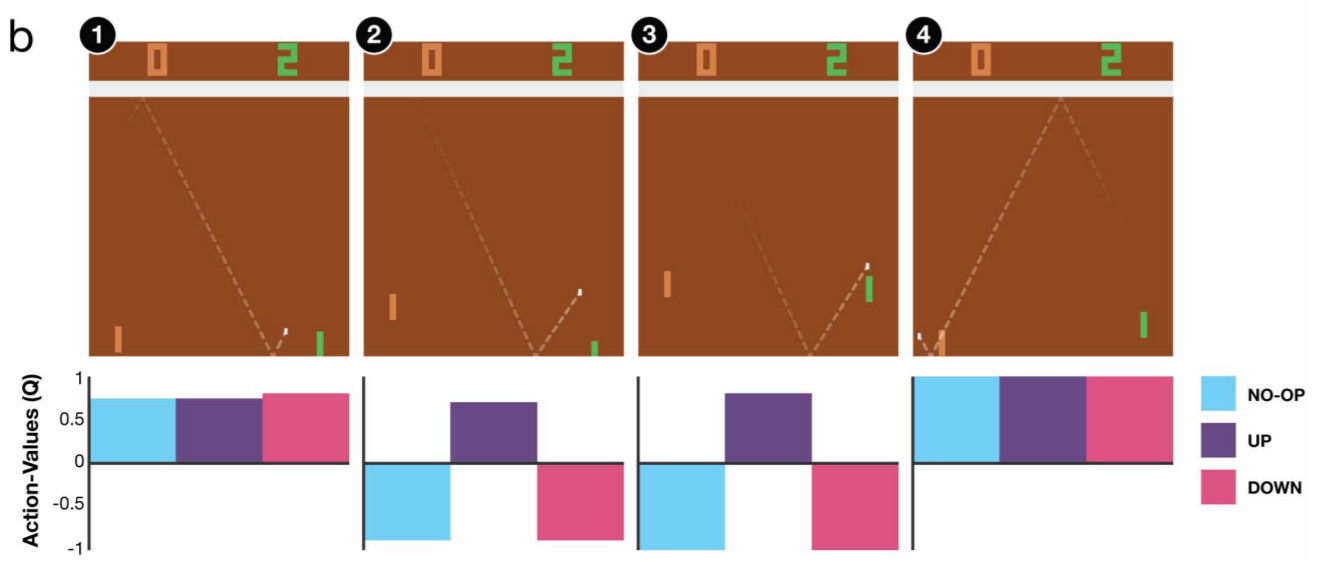
\includegraphics[width=0.9\textwidth]{./imgs/img_rl_qfunction_intuition.png}
    \end{figure}
\end{frame}
%%%%%%%%%%%%%%%%%%%%%%%%%%%%%%%%%%%%%%%%%%%%%%%%%%%%%%%%%%%

\bibliographystyle{apacite}
\bibliography{main}

\end{document}

